\documentclass[11pt]{article}
\usepackage[utf8]{inputenc}
\usepackage{graphicx}
\usepackage{color}
\usepackage[margin=1.in]{geometry}

\setcounter{page}{3}

\begin{document}
\begin{titlepage}
\centering
	
\includegraphics[width=0.30\textwidth]{logo.png}\par\vspace{1cm}
	{\scshape\LARGE Massey University \par}
	\vspace{1cm}
	{\scshape\Large Individual Research: 228.798\par}
	\vspace{1.5cm}
	{\huge\bfseries Literature Review \par}
    \vspace{1cm}
    {\large\bfseries Self morphing soft robotic gripper for the handling and manipulation of delicate produce in horticultural applications\par}
	\vspace{2cm}
	{\large\itshape Dean Gerhardus Venter\par}
	\vspace{2cm}
	{\large\itshape 14074740\par}
	\vfill
	supervised by\par
	Dr. Steven  \textsc{Dirven}
   
	\vfill

% Bottom of the page
	{\large \today \par}
\end{titlepage}
\begin{titlepage}
\tableofcontents
\end{titlepage}
\section{Introduction}
The capability to autonomously grasp objects remain a chalenge, even in the modern day and age since we continually strive to produce a gripper whcih is equally or more effective than the the human hand. There are a wide range of robotic grippers available in industry, all of whcih have different capabilities and purposes. Conventional grippers are currently prodominantly being produced using rigid links, mechanical joints and are mechanically actuated \cite{ilievski2011soft}. However, the conventional methods are not suitable for delicate operations such as minimally invasive surgery or handling delicate objects such as produce in the form of fesh fruit and vegetables, thus soft robotics has been becoming an increasingly popular alternative. The research into soft robotic alternatives is being done in order to produce soft robots which are capable of completing tasks which conventional rigid-bodied robots are incapable of doing such as delicately handling soft items or working alongside humans \cite{bilodeau2015monolithic}.
\\
\newline
Soft robotics is a biologically inspired class of robotics which is produced using non-rigid, elastomer's which have the capability to morph and conform around the object which they are gripping to varying extents\cite{ilievski2011soft,bilodeau2015monolithic,mosadegh2014pneumatic,martinez2013robotic,marchese2015recipe}.The rigidity of the gripper can be altered in order to suit the required application, allowing it to be more complient and have multiple of an infinate degrees of freedom \cite{hassan2015design}. By using soft materials, it allows us to mimic the capability of the soft tissue of animals morphing around the object which is being grasped, thus allowing for the stress being produced in the grasp to be distributed over a larger area, thus reducing the pressure on the object being grasped \cite{ilievski2011soft}. In the case of grasping delicate objects, this capability is highly sought after because it allows for no point loading, thus reducing the risk of damage  during handling.
\\
\newline
There are a wide range of soft grippers which operate differently based on the geometrical layout of the gripper as well as the actuation. Such grippers include:
\begin{itemize}
\item Tendon actuated
\item Pneumatically actuated
\item hydraulically actuated
\item Particle jamming
\end{itemize}
In the following report, each of the different applicable methods will be discussed.
\section{Project Context}
In 2015 the New Zealand horticulture industry estimated the export of fresh and processed fruits to be worth in excess of \$2.14 billion dollars, of which kiwi fruits made up approximately 1,181.9 billion dollars as shown in Figure \ref{fig:Pie} \cite{fresh_facts_2015}. The New Zealand export industry is of the utmost importance to growth of the local economy, thus it is in the interest of all kiwi's to optimise our exports weather it is dairy, horticultural or meats. In the horticulture industry, a major challenge is to harvest the produce efficiently, especially delicate produce such as kiwi fruit and berries. The current method of harvesting delicate produce is mostly manual seasonal labour as well as a small portion of the industry exploring soft robotic options. However, neither of the two current options which are currently being used for harvesting are meeting the efficiency requirements. The issues associated with the current methods are discussed below:
\begin{figure}[h]
\centering
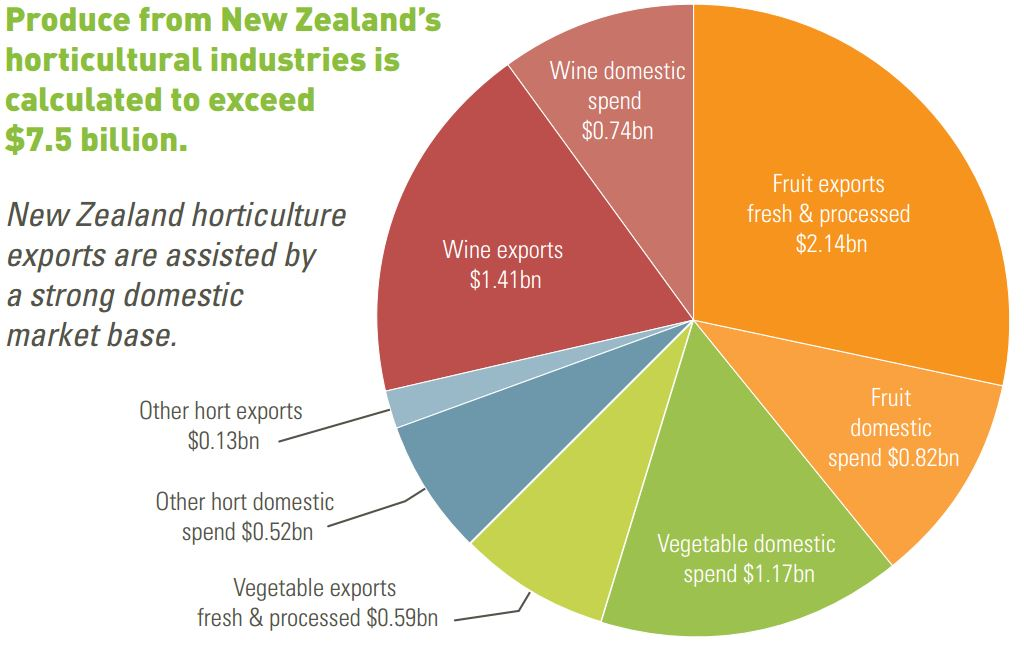
\includegraphics[scale=0.45]{pie_imports}
\caption{New Zealand horticultural exports}
\label{fig:Pie}
\end{figure}
\subsection{Manual seasonal labour}
The kiwi fruit harvesting season in New Zealand is between the months of April and August, meaning that there is not year round harvesting of the fruits. This is a issue due to the fact that it means that the staff which manually harvest the fruits by hand is mostly comprised of seasonal foreign staff whom are working tourists. Thus, virtually no experience can be built by staff, therefore for the initial stages of the harvest, the picking technique is poor, leading to damaged produce and injured staff. In the year dated July 2015 to June 2016, there was a total of 4,084 claims made to the ACC for farm workers whom had sustained a injury caused by Lifting and/or carrying objects. This amounted to a total cost of \$7,283,868 to treat \cite{injury_statistics_tool_2017}. A major contributing factor to this is the sheer size of the loads these staff have to carry, causing their body to be under constant strain as shown in Figure \ref{fig:Picking}.  Both of these factors incur costs for the farmers whom have to pay increasing ACC levy's and loose income due to damaged produce, thus raising the price of the produce leading to a reduction in exports.
\begin{figure}[h]
\centering
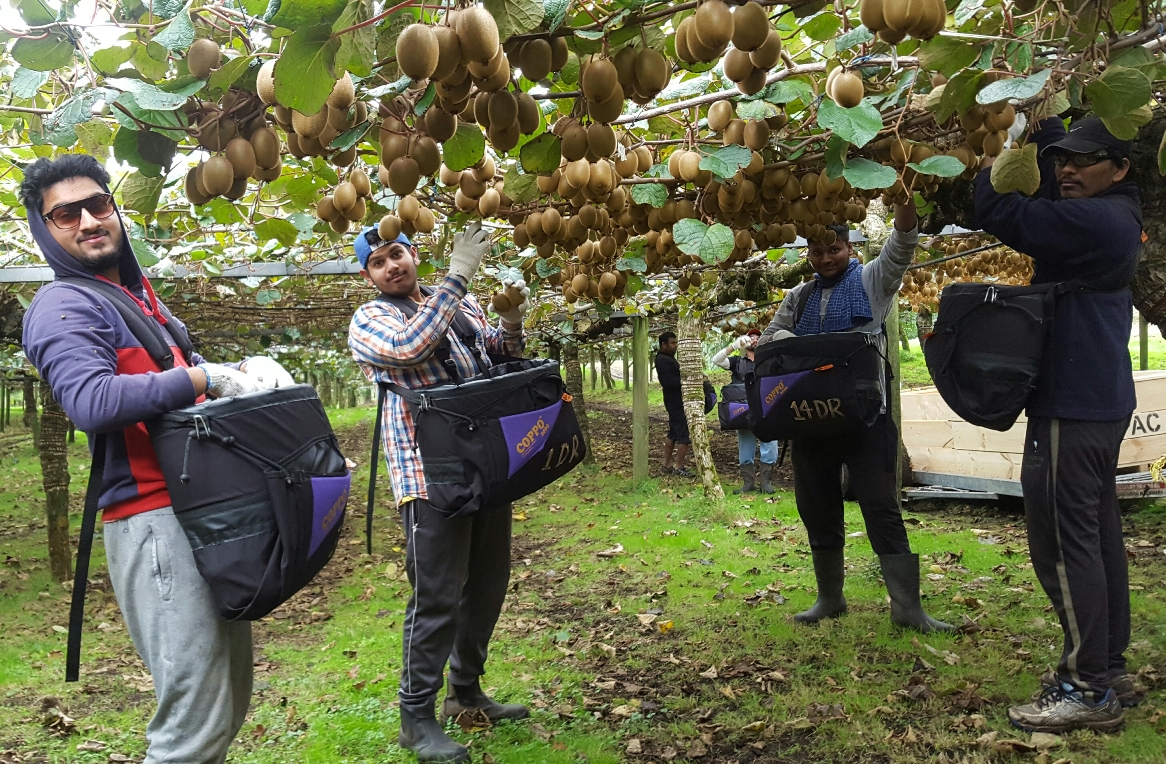
\includegraphics[scale=0.2]{Pickers}
\caption{Seasonal picking staff}
\label{fig:Picking}
\end{figure}


\subsection{Autonomous soft grippers}
Soft robotics is a revolutionary bio-inspired branch of robotics. It incorporates soft technologies which can potentially reduce the mechanical and algoritimic complexity in current robots. It allows robots to have bio inspired capabilities such as flexible interactions in unpredictable environments \cite{kim2013soft}. The current autonomous methods of harvesting the fruits from the vine are very mechanical and often do not have the capability of harvesting the fruit delicately to ensure minimal or no bruising occurs to the specimen. Many of the handling mechanisms currently used grip the fruits too firmly, incorrectly, or do not morph around the shape of the specimen, thus causing damage to the fruit. The most efficient of the current autonomous methods all have a biometric inspired design \cite{hassan2015design}. Thus is due to the fact that the shape of the humanoid hand, leads to optimal picking due to the fact that there is large amounts of surface area and force control. Bruising of fruits can cause the skin to split, leading to the opportunity for bacteria and fungi to enter the fruit. This causes the fruit to spoil at an accelerated rate, thus not being of an acceptable standard for purchase once it has made it to the point of retail .
\\
\newline
Considering the context of the problem which has been discussed above, I propose to conduct research into the harvesting mechanisms of delicate fruits and berries such as kiwifruit with the aim of recommending a soft robotic manipulator which has a success rate of handling produce more efficiently than the current methods used in industry. Since most of the current methods are very mechanical based, this research will be more focused on the biomimetric solutions and it can produce a more effective solution. This project is limited to the end effector of the robot only. It will be designed to be attached onto an existing robot which already has the capability of moving around the orchard as well as manipulating the end effector to be in reach of the fruit or berries. Thus the remainder of the robot is not in the scope of this project.

\section{Past and current Methods}
what are the current methods of gripping delicate objects\cite{mosadegh2014pneumatic}?
\subsection{Mechanical}
Mechanical grippers are grippers which have been produced using rigid links and mechanical joints as well as being mechanically actuated using linear actuators and motors. Mechanical grippers where the shit is the anchient times doe......
Mechanical grippers are very useful at their time when high precision and rapid actuation is required, however their shortcomings are quickly exposed when it comes to handling soft or delicate objects. Due to the mechanical nature, rigid links and joints are required for actuation, thus causing the grippers to be heavy, costly, difficult to control and un-compliant to a array of different shapes \cite{martinez2014soft}. The rigid rigid materials used in production makes it very difficult to develop a mechanical gripper which is capable of handling a range of shapes without causing damage though point loading.

\subsection{Tendon actuated soft gripper}
Tendon actuated soft grippers were the first major leap into the soft robotics field. The as suggested in the name the gripper is actuated using tendon like cables. The cables are often actuated using a range of servo and linear actuators in order to achieve the desired range of motion \cite{marchese2015recipe, dollar2010contact}
\begin{figure}[h]
\centering
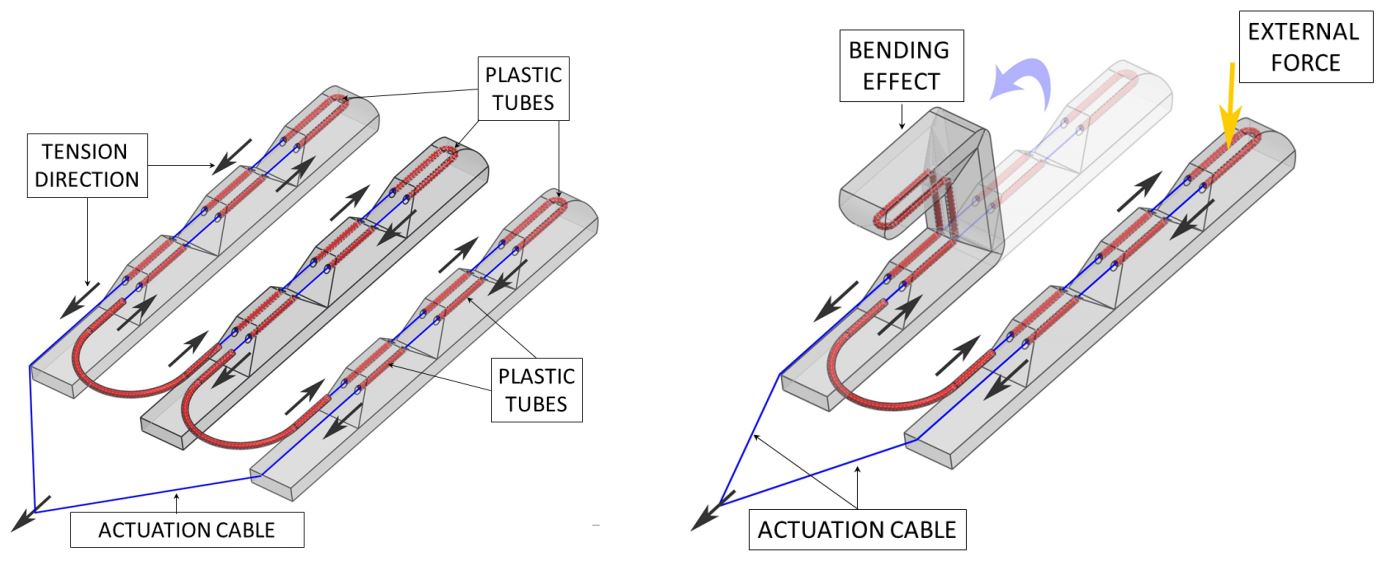
\includegraphics[scale=0.45]{Tendon}
\caption{Tendon actuated soft gripper}
\label{fig:Picking}
\end{figure}
\subsection{Pneumatic under-actuated}
\subsection{Particle jamming}
\section{Most promising current method}
From the analysis which has been done on each of the current options, it was prominent to see that the most promising of the methods was indeed the pneumatically actuated model. This model have been testing using a wide range of configurations and 
\section{Bio-mimetic Options}
\section{Materials}
The material used to produce a compliment soft robotic gripper is very important due to the fact that the material used can completely change the performance of the gripper. In th
\section{Applicable Sensors}
\section{Conclusion}
\bibliographystyle{ieeetr}
\bibliography{Reference}
\end{document}